\begin{figure}[H]
    \centering
    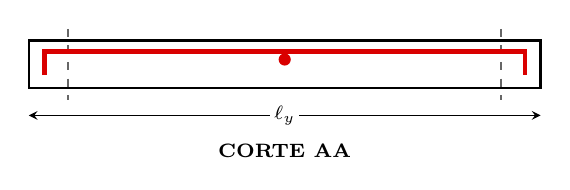
\begin{tikzpicture}[
        scale=1,
        >=stealth,
        contorno/.style={draw=black, thick},
        margem/.style={draw=gray!80!black, thick},
        barra/.style={line width=1.6pt, red!85!black},
        chamada/.style={gray!60!black, thin, dashed},
        cota/.style={<->, thin, black},
        corte/.style={draw=black, dash dot, thick},
        setaCorte/.style={->, very thick, black},
        txt/.style={font=\scriptsize\bfseries, inner sep=1.5pt}
    ]

    % ---------- Parâmetros (planta) ----------
    \def\W{10}      % largura do retângulo maior
    \def\H{6.5}     % altura do retângulo maior (menor que \W)
    \def\m{0.5}     % distância entre os retângulos (= 20 em x e y)
    \def\ext{0.3}   % quanto a barra sai do retângulo menor (< \m)
    \pgfmathsetmacro\cx{\W/2}
    \pgfmathsetmacro\cy{\H/2}
    \pgfmathsetmacro\xa{\cx+1.5}   % posição do corte AA (vertical)
    \pgfmathsetmacro\yb{\cy-1.2}   % posição do corte BB (horizontal)

    %\node[txt] at (\cx,-1.2) {PLANTA DA LAJE};

    % ========== 2. CORTE BB (largura = \W) ==========
    \def\t{0.6}      % espessura da laje no desenho
    \def\dl{0.14}    % posição da armadura (d')
    \def\gh{0.3}     % gancho
    \def\yTop{-3.2}  % topo da laje no corte BB

    % ========== 3. CORTE AA (largura = \H) ==========
    \def\yTopA{-6.4}
    \draw[contorno] (0,\yTopA) rectangle (\H,\yTopA-\t);
    \draw[margem, dashed] (\m,\yTopA+0.15) -- (\m,\yTopA-\t-0.15);
    \draw[margem, dashed] (\H-\m,\yTopA+0.15) -- (\H-\m,\yTopA-\t-0.15);
    % barra secundária (vertical na planta) em comprimento
    \draw[barra] (\m-\ext,\yTopA-\dl-\gh) -- (\m-\ext,\yTopA-\dl)
                 -- (\H-\m+\ext,\yTopA-\dl) -- (\H-\m+\ext,\yTopA-\dl-\gh);
    % barra principal em ponto
    \fill[red!85!black] (\cy,\yTopA-\dl-0.1) circle (2.2pt);
    \draw[cota] (0,\yTopA-\t-0.35) -- (\H,\yTopA-\t-0.35)
        node[midway, fill=white, txt] {$\ell_y$};
    \node[txt] at (\H/2,\yTopA-\t-0.8) {CORTE AA};

    \end{tikzpicture}
    %\caption{Planta da laje e cortes AA e BB}
\end{figure}